\documentclass[aspectratio=169,11pt,hyperref={colorlinks=true}]{beamer}
\usetheme{boxes}
\setbeamertemplate{navigation symbols}{}
\definecolor{openstack}{RGB}{149,0,4}
\setbeamercolor{titlelike}{fg=openstack}
\setbeamercolor{structure}{fg=openstack}
\hypersetup{colorlinks,urlcolor=openstack}
\setbeamertemplate{footline}[frame number]
% Inserting graphics
\usepackage{graphicx}
% Side-by-side figures, etc
\usepackage{subfigure}
% Code snippits
\usepackage{listings}
% Color stuff
\usepackage{color}
\usepackage{amsmath}
\usepackage{tikz}
\usepackage{tipa}
\newcommand\RBox[1]{%
  \tikz\node[draw,rounded corners,align=center,] {#1};%
}
\usepackage{hyperref}
%\usecolortheme{buzz}
%\usecolortheme{wolverine}
%\usetheme{Boadilla}
\usepackage[T1]{fontenc}

\definecolor{mygreen}{rgb}{0,0.6,0}
\definecolor{mygray}{rgb}{0.5,0.5,0.5}
\definecolor{mymauve}{rgb}{0.58,0,0.82}

\lstset{ %
  backgroundcolor=\color{white},   % choose the background color; you must add \usepackage{color} or \usepackage{xcolor}
  breakatwhitespace=false,         % sets if automatic breaks should only happen at whitespace
  breaklines=true,                 % sets automatic line breaking
  captionpos=b,                    % sets the caption-position to bottom
  commentstyle=\color{openstack},  % comment style
  extendedchars=true,              % lets you use non-ASCII characters; for 8-bits encodings only, does not work with UTF-8
  keepspaces=true,                 % keeps spaces in text, useful for keeping indentation of code (possibly needs columns=flexible)
  keywordstyle=\color{blue},       % keyword style
  otherkeywords={*,...},           % if you want to add more keywords to the set
  numbersep=5pt,                   % how far the line-numbers are from the code
  numberstyle=\tiny\color{mygray}, % the style that is used for the line-numbers
  rulecolor=\color{black},         % if not set, the frame-color may be changed on line-breaks within not-black text (e.g. comments (green here))
  showspaces=false,                % show spaces everywhere adding particular underscores; it overrides 'showstringspaces'
  showstringspaces=false,          % underline spaces within strings only
  showtabs=false,                  % show tabs within strings adding particular underscores
  stringstyle=\color{openstack},   % string literal style
}

\setbeamerfont{caption}{series=\normalfont,size=\fontsize{6}{8}}
\setbeamertemplate{caption}{\raggedright\insertcaption\par}

\setlength{\abovecaptionskip}{0pt}
\setlength{\floatsep}{0pt}

\author[Andrea Frittoli]{%
    \texorpdfstring{
        \begin{columns}
            \column{.45\linewidth}
            \centering
            Andrea Frittoli\\
            \href{mailto:andrea.frittoli@hpe.com}{andrea.frittoli@hpe.com}\\
            \texttt{andreaf on Freenode}
        \end{columns}
   }
   {Andrea Frittoli}
}
\date{Apr 25, 2016}

\title[Tempest Stable Interfaces for OpenStack Integration Testing
\hspace{2em}\insertframenumber/\inserttotalframenumber]{Tempest Stable Interfaces for OpenStack Integration Testing}

\begin{document}

{
\setbeamertemplate{background canvas}{
\includegraphics[width=\paperwidth,height=\paperheight]{background_title.png}}
\setbeamertemplate{footline}{}
\begin{frame}[noframenumbering]
    \setbeamercolor{titlelike}{fg=white}
    \setbeamercolor{structure}{fg=white}
    \setbeamercolor{normal text}{fg=white}
    \hypersetup{colorlinks,urlcolor=white}
    \setbeamercolor{author}{fg=white}
    \setbeamercolor{date}{fg=white}
    \setbeamercolor{background}{bg=openstack}
    \titlepage{}
    \centering
    \href{https://github.com/andreafrittoli/templest\_stable\_interfaces}{https://github.com/andreafrittoli/templest\_stable\_interfaces}
\end{frame}
}

\section{Logistics}
\begin{frame}[c]
    \frametitle{Neutron or Newton}
    \begin{center}
        \Huge \textipa{/"nju:t(r)\textturnscripta{}n/}
    \end{center}
\end{frame}

\section{What is OpenStack QA?}
\begin{frame}
    \frametitle{What is OpenStack QA?}
    \begin{itemize}
     \item Official Mission Statement:\\
         \textit{Develop, maintain, and initiate tools and plans to ensure
the upstream stability and quality of OpenStack, and its release readiness at
any point during the release cycle.}
    \end{itemize}
\end{frame}

\begin{frame}
    \frametitle{Current QA Projects}
    \begin{itemize}
        \item{eslint-config-openstack}
        \item{bashate}
        \item{hacking}
        \item{tempest}
        \item{tempest-lib (deprecated)}
        \item{grenade}
        \item{devstack}
        \item{devstack-plugin-ceph}
        \item{devstack-vagrant}
        \item{stackviz}
        \item{openstack-health dashboard}
        \item{os-testr}
        \item{devstack-plugin-cookiecutter}
        \item{tempest-plugin-cookiecutter}
        \item{os-performance-tools}
    \end{itemize}
\end{frame}

\section{Tempest}
\begin{frame}[c]
    \frametitle{What is Tempest}
    \begin{center}
    	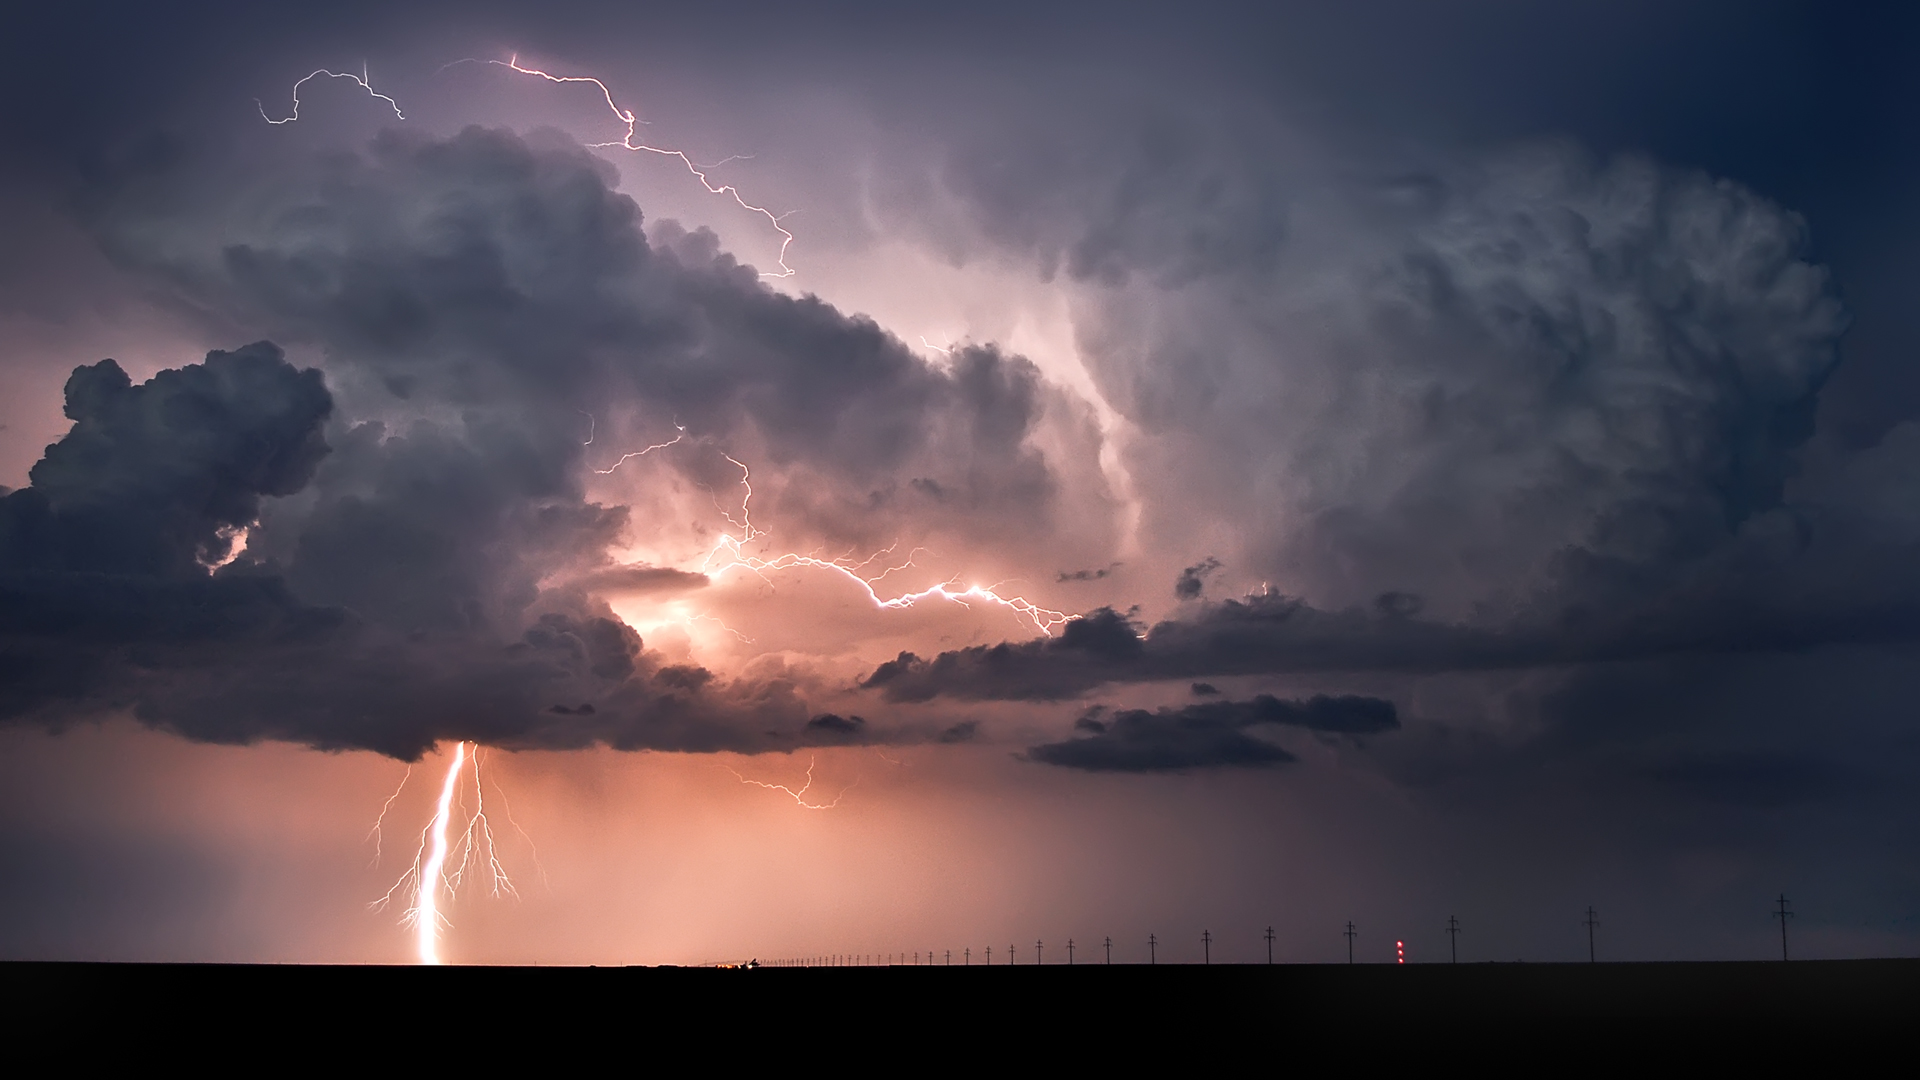
\includegraphics[width=1.0\textwidth]{tempest.jpg}
    \end{center}
\end{frame}

\begin{frame}[c]
    \frametitle{Tempest in the Big Tent}
    \begin{itemize}
        \item tempest\_lib or tempest.lib
        \item tempest plugins
    \end{itemize}
\end{frame}

\begin{frame}
    \frametitle{Current Projects QA directly supports in-tree}
    \begin{itemize}
        \item Keystone
        \item Nova
        \item Glance
        \item Cinder
        \item Neutron
        \item Swift
    \end{itemize}
    \begin{itemize}
        \item{Tests executed in integrated-gate jobs}
    \end{itemize}
\end{frame}

\section{Growth of tests out of Tempest Tree}
\begin{frame}[c]
    %\frametitle{Integration Tests in and out of tree}
    \begin{center}
        \large Where do other Tempest based tests live in OpenStack?
    \end{center}
\end{frame}

\begin{frame}
    \frametitle{Integration Tests outside of Tempest tree}
    \begin{itemize}
        \item{Tempest Plugins (29)}
        \item{CLI tests for clients (16)}
        \item{Other functional/integration tests}
    \end{itemize}
    \text{ }
    \begin{itemize}
        \item{Not executed against tempest}
        \item{Should only use tempest stable interfaces}
    \end{itemize}
\end{frame}

\begin{frame}
    \frametitle{Tempest Plugins at the end of Liberty}
    \begin{figure}[p]
    	\centering
    	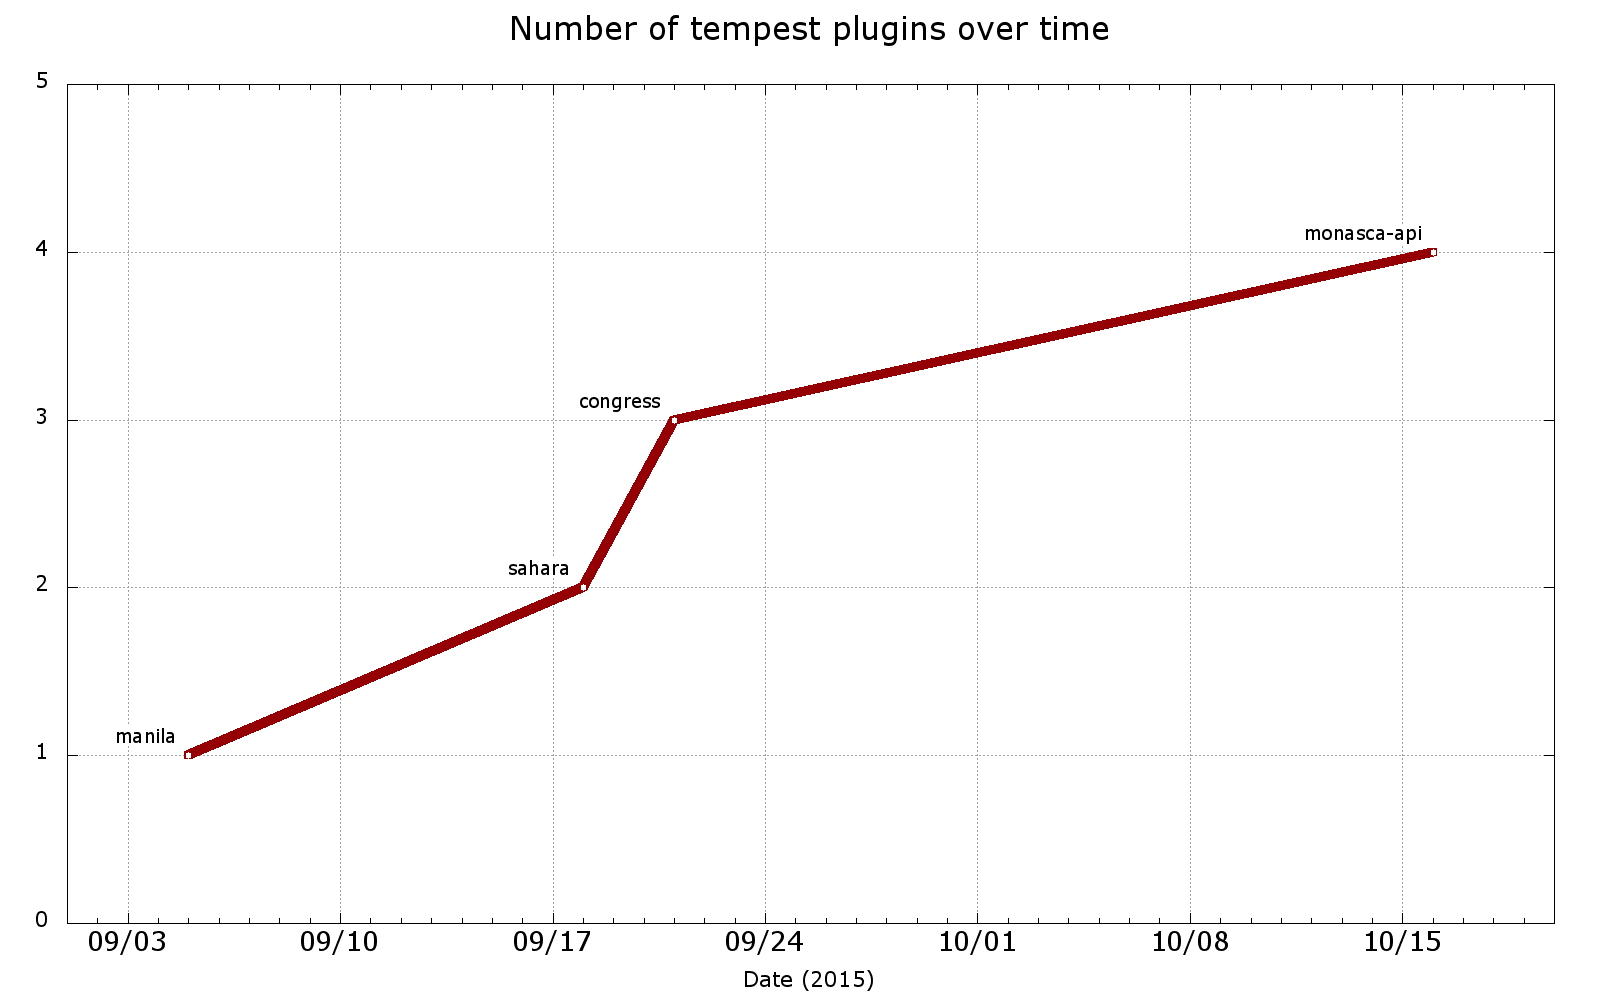
\includegraphics[width=0.7\textwidth]{tempest-plugins-old.png}
        \caption{Source: git blame -L '/\^{}tempest/,+1' setup.cfg | awk '\{print \$1\}' | xargs git log -1 --format=\%cd --date=short}
    \end{figure}
\end{frame}

\begin{frame}
    \frametitle{Tempest Plugins over time}
    \begin{figure}[p]
    	\centering
    	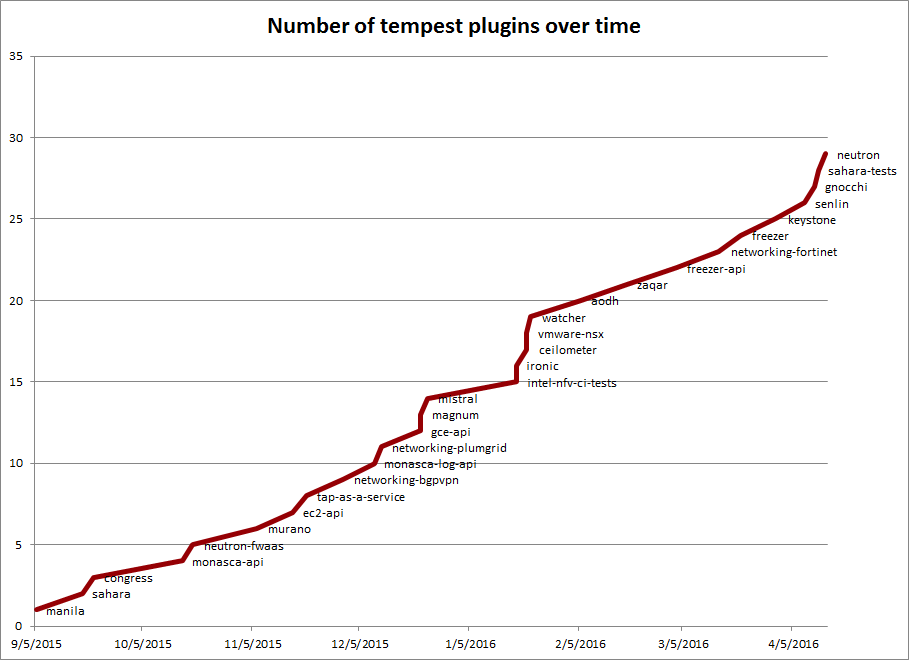
\includegraphics[width=0.7\textwidth]{tempest-plugins.png}
        \caption{Source: git blame -L '/\^{}tempest/,+1' setup.cfg | awk '\{print \$1\}' | xargs git log -1 --format=\%cd --date=short}
    \end{figure}
\end{frame}

\begin{frame}
    \frametitle{CLI Tests over time}
    \begin{figure}[p]
    	\centering
    	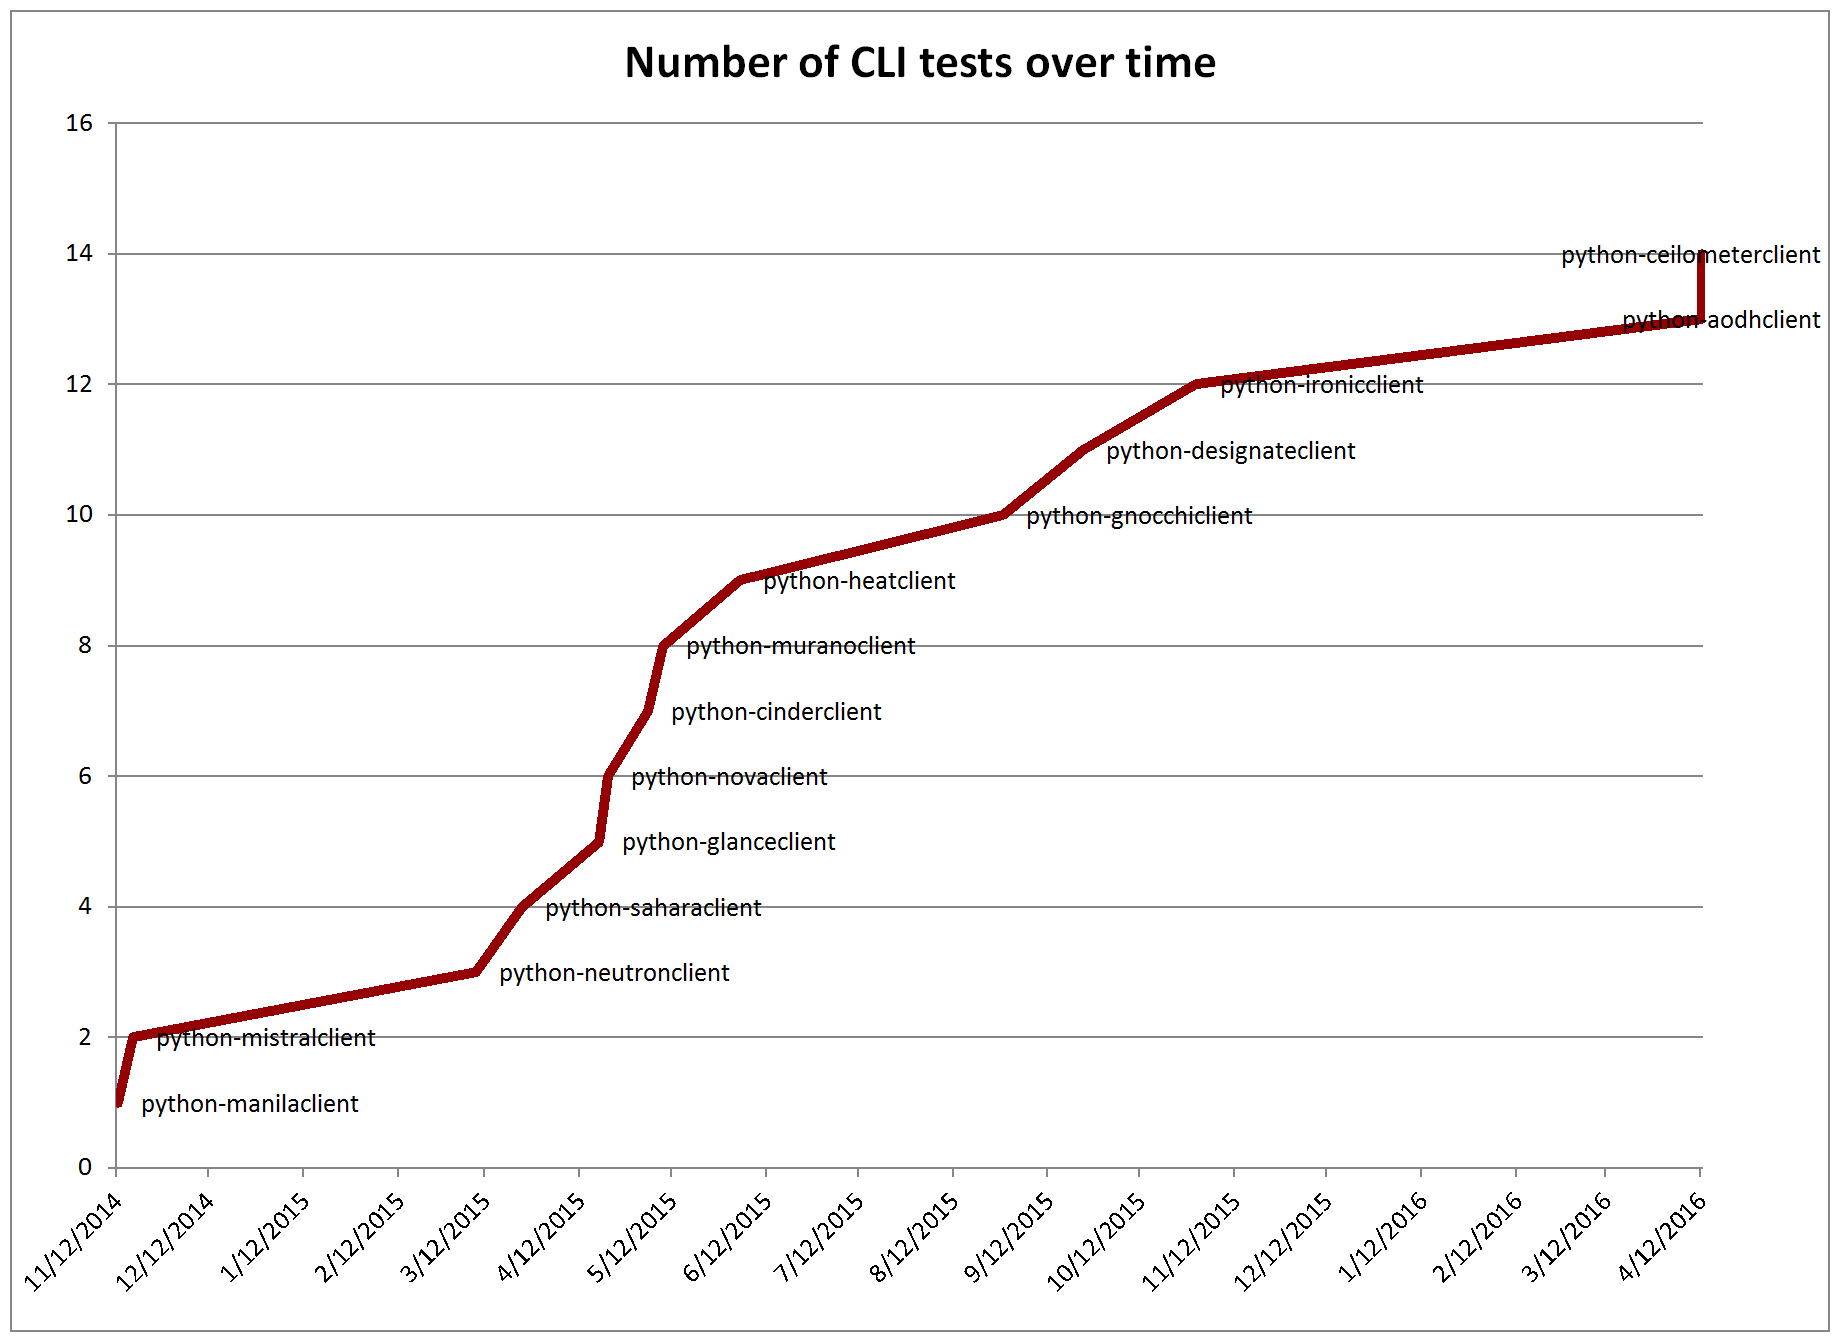
\includegraphics[width=0.7\textwidth]{cli-tests.png}
        \caption{Source: git blame -L '/\^{}(from|import) tempest[\_.]+lib.cli/,+1' *.py}
    \end{figure}
\end{frame}

\begin{frame}
    \frametitle{Other Tempest Tests}
    \begin{itemize}
        \item{WIP Tempest Plugins}
            \begin{itemize}
                \item{kingbird}
                \item{vitrage}
            \end{itemize}
    \end{itemize}
    \begin{itemize}
        \item{Tempest Tests (potential plugins)}
            \begin{itemize}
                \item{blazar}
                \item{designate}
                \item{networking-l2gw}
                \item{networking-vsphere}
                \item{neutron-lbaas}
                \item{neutron-vpnaas}
            \end{itemize}
    \end{itemize}
\end{frame}

\begin{frame}
    \frametitle{Functional/Integration Tests}
    \begin{itemize}
        \item{cerberus (rest\_client, auth, clients)}
        \item{cue (rest\_client, test base class)}
        \item{solum (rest\_client, auth)}
    \end{itemize}
    \begin{itemize}
        \item{astara (utils)}
        \item{barbican (utils)}
        \item{python-keystoneclient (test base class)}
        \item{python-openstackclient (utils)}
        \item{tacker (test base class)}
    \end{itemize}
\end{frame}

\begin{frame}[c]
    %\frametitle{Integration Tests in and out of tree}
    \begin{center}
        \large What are Tempest (Stable) Interfaces, how are they used?
    \end{center}
\end{frame}

\section{Tempest Interfaces}
\begin{frame}
    \frametitle{Tempest Stable APIs}
    \begin{itemize}
        \item{Common: rest client, microversion, ssh client, utils}
        \item{Service clients: identity, network, compute}
        \item{Authentication providers}
        \item{CLI test framework}
        \item{Decorators, exceptions}
        \item{Base test class}
        \item{Commands: check\_uuid, skip tracker}
    \end{itemize}
\end{frame}

\begin{frame}
    \frametitle{Tempest Stable APIs}
    \begin{figure}[p]
    	\centering
    	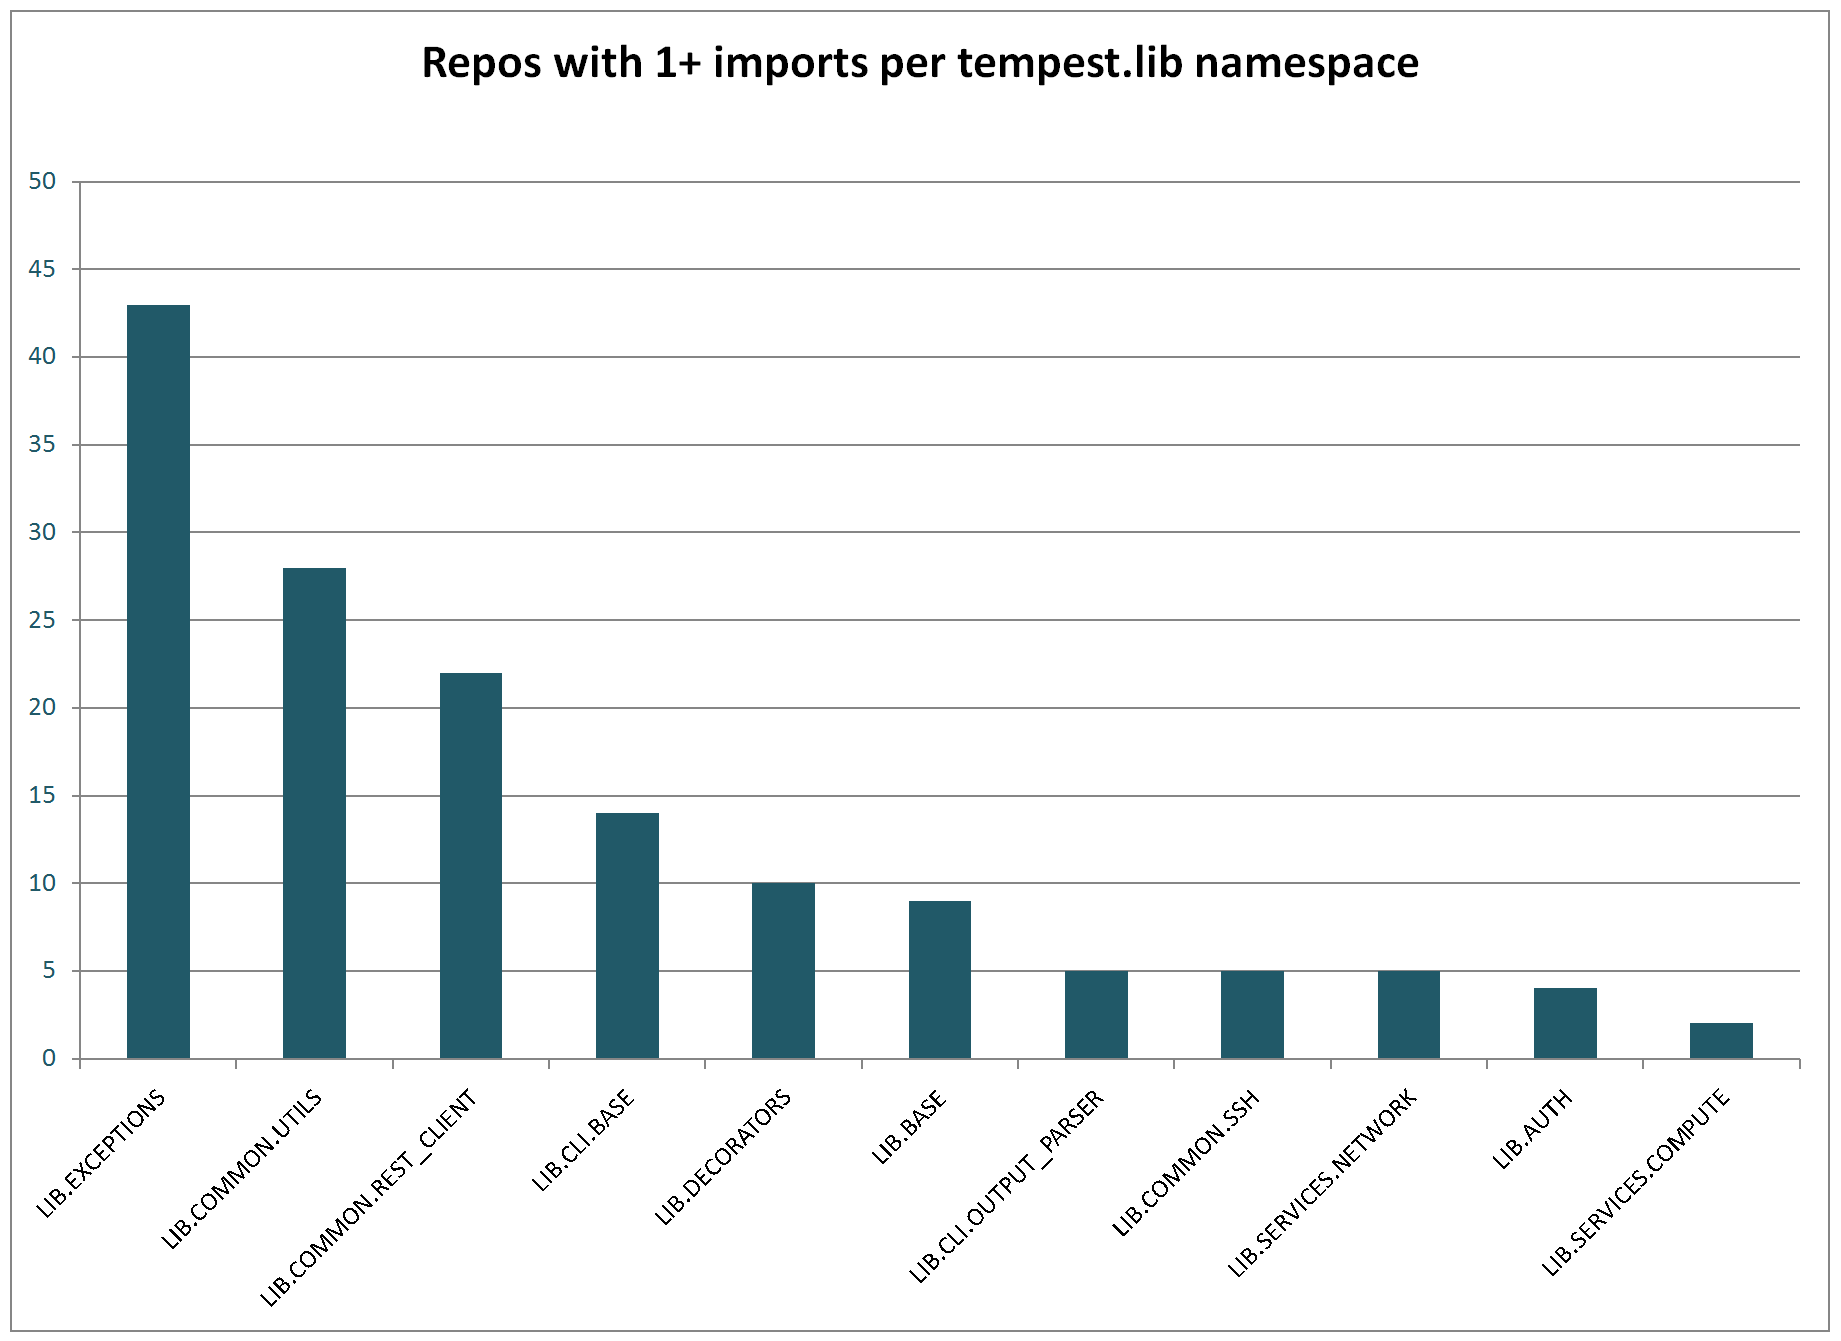
\includegraphics[width=0.7\textwidth]{lib-imports.png}
    	\caption{Source: codesearch.openstack.org}
    \end{figure}
\end{frame}

\begin{frame}
    \frametitle{Tempest Internal APIs planned to become Stable}
    \begin{itemize}
        \item{Service clients: volume, image, object-storage}
        \item{Credential providers}
        \item{Client manager}
        \item{Plugin}
    \end{itemize}
\end{frame}

\begin{frame}
    \frametitle{Tempest Internal APIs}
    \begin{figure}[p]
    	\centering
    	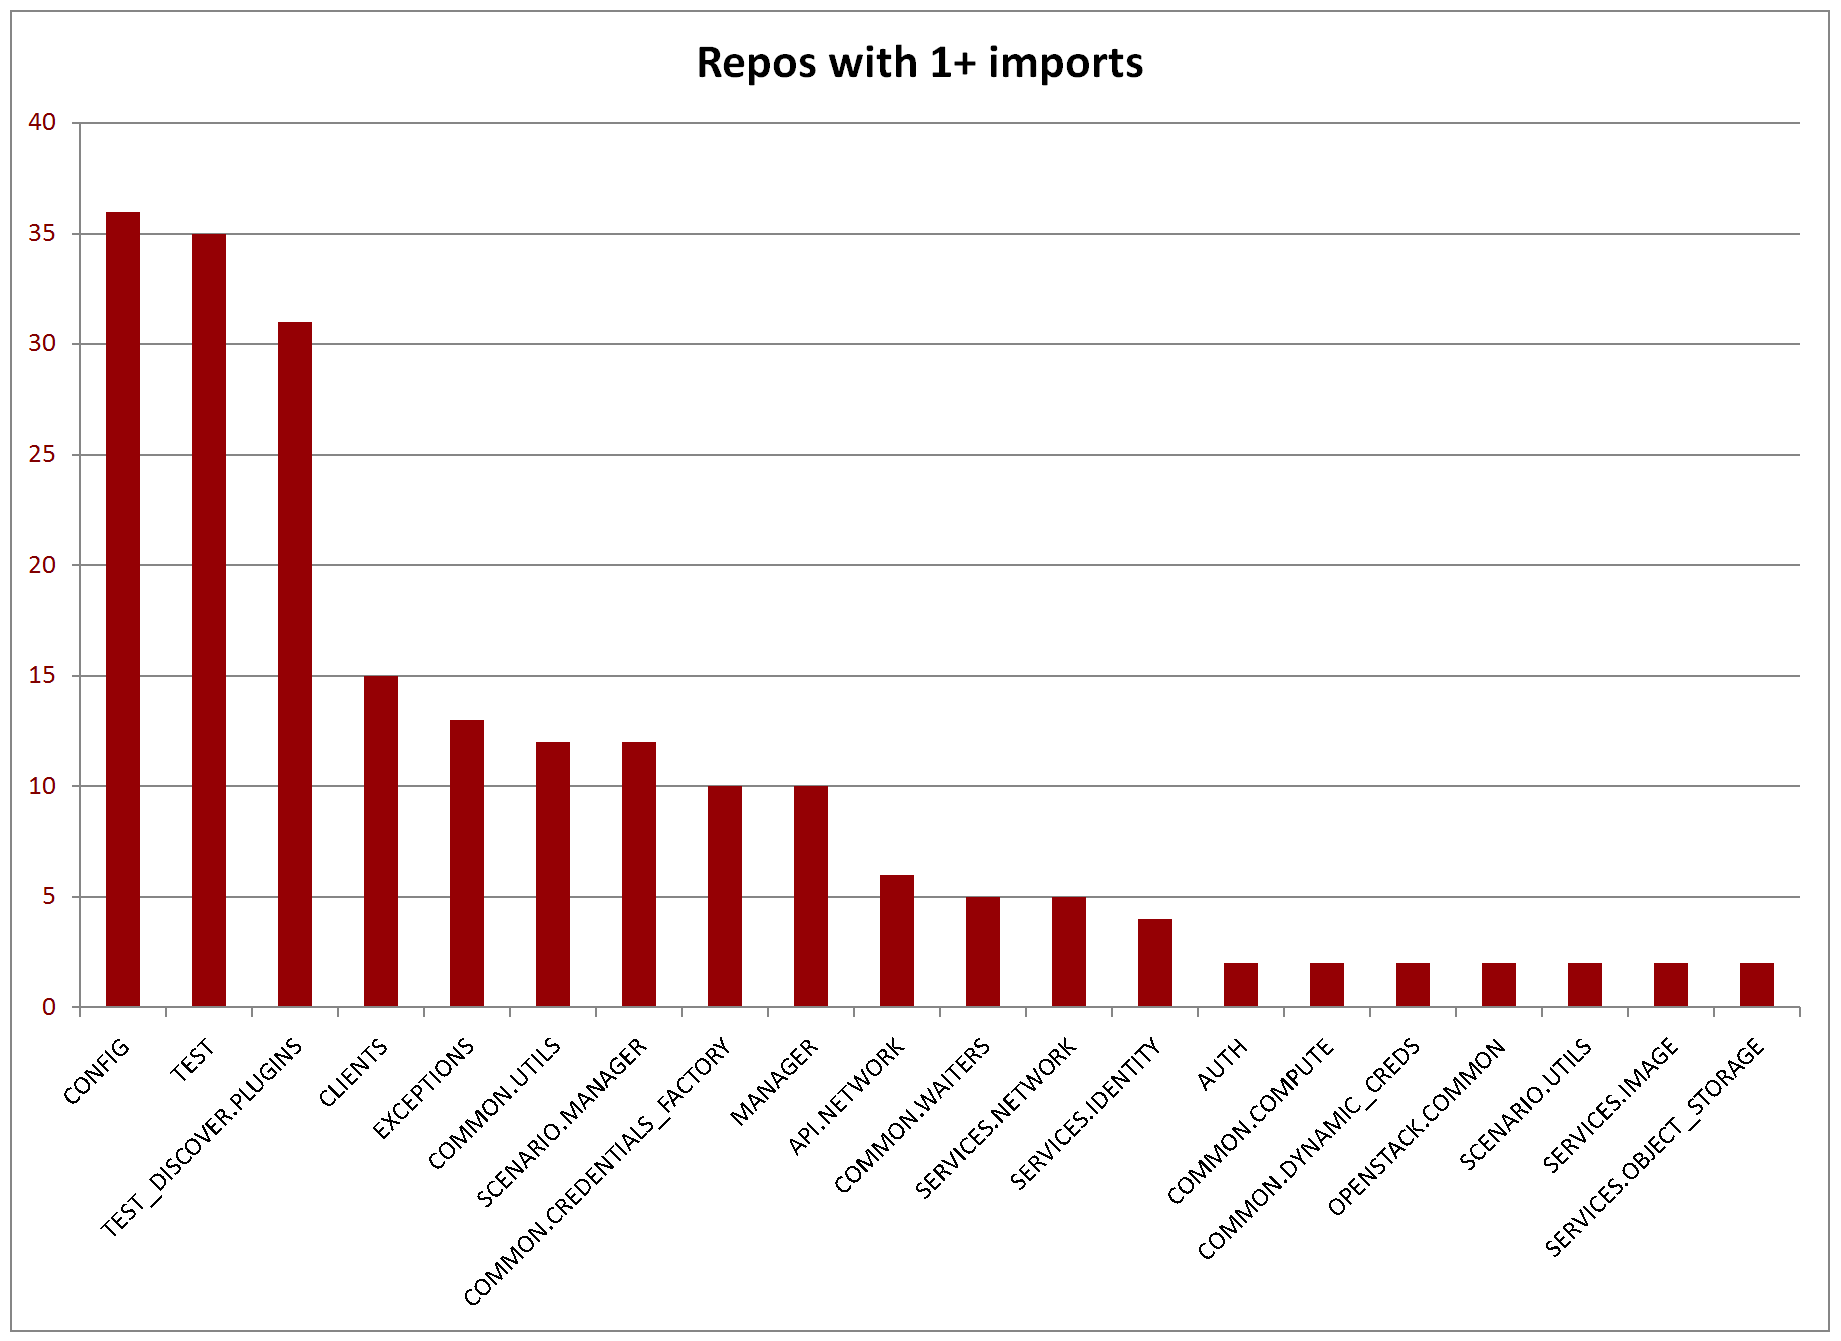
\includegraphics[width=0.7\textwidth]{tempest-imports.png}
    	\caption{Source: codesearch.openstack.org}
    \end{figure}
\end{frame}

\section{Writing Plugins}
\begin{frame}[c]
    %\frametitle{Tempest Plugins}
    \begin{center}
        \large How to use these interfaces to write a Tempest plugin?
    \end{center}
\end{frame}

\begin{frame}
    \frametitle{Tempest Plugins Interface}
    \begin{itemize}
        \item Integrates external tests into a tempest run
        \item Unifies configuration between plugin(s) and in-tree
        \item Integrates custom service clients (planned)
    \end{itemize}
    \begin{itemize}
    	\item{Based on stevedore extension manager}
    	\item{Automatically discovered when installed}
    \end{itemize}
\end{frame}

\begin{frame}
    \frametitle{Tempest Plugins Interface}
    \lstinputlisting[basicstyle=\tiny,language=Python]{code/manila_plugin.py}
    \begin{itemize}
        \item \tiny Full code at: \href{http://git.openstack.org/cgit/openstack/manila/tree/manila_tempest_tests/plugin.py}{http://git.openstack.org/cgit/openstack/manila/tree/manila\_tempest\_tests/plugin.py}
    \end{itemize}
\end{frame}

\begin{frame}
    \frametitle{Rest Client and Service Clients}
    \begin{itemize}
        \item ReST API Calls with different HTTP methods
        \item Decorate requests using supplied auth provider
        \item Validate HTTP return codes
        \item Handle HTTP non-2xx return codes as custom exceptions
    \end{itemize}
    \begin{itemize}
        \item Methods for API calls
        \item Minimal response body parsing
        \item Pass any parameter to API calls
    \end{itemize}
\end{frame}

\begin{frame}
    \frametitle{Rest Client and Service Clients}
    \lstinputlisting[basicstyle=\tiny,language=Python]{code/ceilometer_client.py}
    \begin{itemize}
        \item \tiny Full code at: \href{http://git.openstack.org/cgit/openstack/ceilometer/tree/ceilometer/tests/tempest/service/client.py}{http://git.openstack.org/cgit/openstack/ceilometer/tree/ceilometer/tests/tempest/service/client.py}
    \end{itemize}
\end{frame}

\begin{frame}
    \frametitle{Authentication Layer}
    \begin{itemize}
        \item Credentials object
        \item Select endpoints from the catalogue
        \item Decorate requests with identity v2 and v3 auth data
        \item Inject alternate auth data
    \end{itemize}
\end{frame}

\begin{frame}
    \frametitle{Authentication Layer}
    \lstinputlisting[basicstyle=\tiny,language=Python]{code/auth_provider.py}
    \begin{itemize}
        \item \tiny Full code at: \href{http://git.openstack.org/cgit/openstack/tempest/tree/tempest/manager.py}{http://git.openstack.org/cgit/openstack/tempest/tree/tempest/manager.py}
    \end{itemize}
\end{frame}

\begin{frame}
    \frametitle{Client Managers}
    \begin{itemize}
        \item One object to access all service clients
        \item Bound to a set of credentials
        \item Hide the complexity of the auth layer
        \item Not yet in the lib namespace (WIP)
    \end{itemize}
    \begin{itemize}
        \item Stable interface to register service clients from plugins
        \item Lazy loading of clients
    \end{itemize}
\end{frame}

\begin{frame}
    \frametitle{Client Managers}
     \lstinputlisting[basicstyle=\tiny,language=Python]{code/neutron_manager.py}
    \begin{itemize}
        \item \tiny Full code at: \href{http://git.openstack.org/cgit/openstack/neutron/tree/neutron/tests/tempest/api/clients.py}{http://git.openstack.org/cgit/openstack/neutron/tree/neutron/tests/tempest/api/clients.py}
    \end{itemize}
\end{frame}

\begin{frame}
    \frametitle{Credential Providers}
    \begin{itemize}
        \item Supply test cases with credentials
        \item Manage multiple test account for parallel test execution
        \item Manage account specific network resources
        \item Not yet in the lib namespace (WIP)
    \end{itemize}
    \begin{itemize}
        \item Dynamic Credential Provider
        \item Preprovisioned Credential Provider
    \end{itemize}
\end{frame}

\begin{frame}
    \frametitle{Testing microversions}
    \begin{itemize}
        \item Define acceptable microversion range for test class
        \item Match configured microversion range with tests
        \item Select microversion to be sent via API
    \end{itemize}
\end{frame}

\begin{frame}
    \frametitle{Testing microversions}
    \lstinputlisting[basicstyle=\tiny,language=Python]{code/microversion.py}
    \begin{itemize}
        \item \tiny Full code at: \href{http://git.openstack.org/cgit/openstack/tempest/tree/tempest/api/compute/base.py}{http://git.openstack.org/cgit/openstack/tempest/tree/tempest/api/compute/base.py}
    \end{itemize}
\end{frame}

\begin{frame}
    \frametitle{Miscellaneous Utils}
    \begin{itemize}
        \item Generate random test data
        \item SSH client
        \item Skip decorators
        \item Test Attributes (not yet stable)
    \end{itemize}
\end{frame}

\section{Writing CLI Tests}
\begin{frame}[c]
    %\frametitle{CLI Tests}
    \begin{center}
        \large Which interfaces do you need to implement CLI tests?
    \end{center}
\end{frame}

\begin{frame}
    \frametitle{CLI Tests Interfaces}
    \begin{itemize}
        \item An \emph{execute} command to drive clients via CLI
        \item A \emph{CLIClient} class that wraps \emph{execute} for clients
        \item An \emph{output\_parser} module with helpers to parse clients output
        \item A \emph{ClientTestBase} class with clients and output parsers
    \end{itemize}
\end{frame}

\begin{frame}
    \frametitle{CLI Tests Interfaces}
    \lstinputlisting[basicstyle=\tiny,language=Python]{code/mistral_cli.py}
    \begin{itemize}
        \item \tiny Full code at: \href{http://git.openstack.org/cgit/openstack/python-mistralclient/tree/mistralclient/tests/functional/cli/base.py}{http://git.openstack.org/cgit/openstack/python-mistralclient/tree/mistralclient/tests/functional/cli/base.py}
    \end{itemize}
\end{frame}

\section{Usage of Tempest APIs in OpenStack}
\begin{frame}[c]
    %\frametitle{Usage of Tempest APIs in OpenStack}
    \begin{center}
        \large How are Tempest interfaces used today in OpenStack?
    \end{center}
\end{frame}

\section{More Information}
\begin{frame}
\frametitle{Where to get more information}
    \begin{itemize}
        \item Tempest Stable Interfaces Docs: \href{http://docs.openstack.org/developer/tempest/library.html}{http://docs.openstack.org/developer/tempest/library.html}
        \item Tempest Plugin Docs: \href{http://docs.openstack.org/developer/tempest/plugin.html}{http://docs.openstack.org/developer/tempest/plugin.html}
        \item Tempest External Plugins Presentation: \href{https://github.com/mtreinish/external_plugins}{https://github.com/mtreinish/external\_plugins}
        \item \#openstack-qa on Freenode
    \end{itemize}
\end{frame}

\section{Questions}
\begin{frame}[c]
    %\frametitle{Questions?}
    \begin{center}
        \Huge Questions?
    \end{center}
\end{frame}

%\section{Extra Info}
\end{document}
